\begin{infocard}{Triángulos rectángulos}
    Para un triángulo rectangulo, el cuadrado de la hipotenusa $H$ es igual a la suma de los cuadrados de los catetos opuesto $CO$ y adyacente $CA$:
    \[H^2=CO^2+CA^2\]
    % \end{minipage}\hfill
    % \begin{minipage}{0.3\textwidth}
    % \begin{figure}[H]
    %     \centering
    %     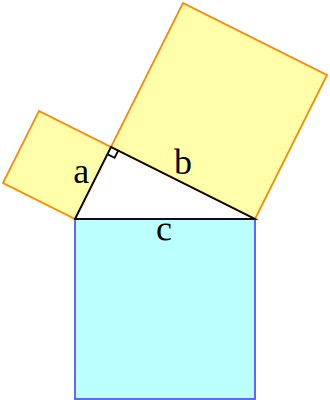
\includegraphics[width=0.55\linewidth]{../images/pythagorean_right_angle}
    %     \caption{}
    %     \label{fig:pythagorean_right_angle}
    % \end{figure}
    % \end{minipage}
    \newcommand{\pythagwidth}{2.2cm}
    \newcommand{\pythagheight}{1.3cm}
    \centering
    \begin{tikzpicture}

        \coordinate  (A) at (0, 0);
        \coordinate  (B) at (0, \pythagheight);
        \coordinate (C) at (-\pythagwidth, 0);

        \coordinate (D1) at (-\pythagheight, \pythagheight + \pythagwidth);
        \coordinate (D2) at (-\pythagheight - \pythagwidth, \pythagwidth);

        \draw [thick] (A) -- node [below] {CA} (C) -- node [above left] {H} (B) -- node [above right] {CO} (A);
        \draw[fill=lightgray, thick] (C) -- ++(0:0.8cm) arc (0:90-atan2(\pythagwidth,\pythagheight):0.8cm) node at ($(20:0.5cm)+(C)$) {$\theta$} -- cycle;

        \newcommand{\ranglesize}{0.3cm}
        \draw (A) -- ++ (0, \ranglesize) -- ++ (-\ranglesize, 0) -- ++ (0, -\ranglesize);

        \draw [dashed] (A) -- node [below] {} ++ (-\pythagwidth, 0)
        -- node [right] {} ++ (0, -\pythagwidth)
        -- node [above] {} ++ (\pythagwidth, 0)
        -- node [left] {} ++ (0, \pythagwidth);

        \draw [dashed] (A) -- node [right] {} ++ (0, \pythagheight)
        -- node [below] {} ++ (\pythagheight, 0)
        -- node [left] {} ++ (0, -\pythagheight)
        -- node [above] {} ++ (-\pythagheight, 0);

        \draw [dashed] (C) -- node [above left] {} (B)
        -- node [below left] {} (D1)
        -- node [below right] {} (D2)
        -- node [above right] {} (C);
    \end{tikzpicture}


    Además, existen 3 funciones trigonométricas:
    \[
        \sin(\theta)  = \frac{\text{CO}}{\text{H}} \quad
        \cos(\theta)  = \frac{\text{CA}}{\text{H}} \quad
        \tan(\theta)  = \frac{\text{CO}}{\text{CA}}
    \]

\end{infocard}
